\chapter{Time complexity}

\index{time complexity}

The efficiency of algorithms is important in competitive programming.
Usually, it is easy to design an algorithm
that solves the problem slowly,
but the real challenge is to invent a
fast algorithm.
If the algorithm is too slow, it will get only
partial points or no points at all.

The \key{time complexity} of an algorithm
estimates how much time the algorithm will use
for some input.
The idea is to represent the efficiency
as an function whose parameter is the size of the input.
By calculating the time complexity,
we can find out whether the algorithm is good enough
without implementing it.

\section{Calculation rules}

The time complexity of an algorithm
is denoted $O(\cdots)$
where the three dots represent some
function.
Usually, the variable $n$ denotes
the input size.
For example, if the input is an array of numbers,
$n$ will be the size of the array,
and if the input is a string,
$n$ will be the length of the string.

\subsubsection*{Loops}

A common reason why an algorithm is slow is
that it contains many loops that go through the input.
The more nested loops the algorithm contains,
the slower it is.
If there are $k$ nested loops,
the time complexity is $O(n^k)$.

For example, the time complexity of the following code is $O(n)$:
\begin{lstlisting}
for (int i = 1; i <= n; i++) {
    // code
}
\end{lstlisting}

And the time complexity of the following code is $O(n^2)$:
\begin{lstlisting}
for (int i = 1; i <= n; i++) {
    for (int j = 1; j <= n; j++) {
        // code
    }
}
\end{lstlisting}

\subsubsection*{Order of magnitude}

A time complexity does not tell us the exact number
of times the code inside a loop is executed,
but it only shows the order of magnitude.
In the following examples, the code inside the loop
is executed $3n$, $n+5$ and $\lceil n/2 \rceil$ times,
but the time complexity of each code is $O(n)$.

\begin{lstlisting}
for (int i = 1; i <= 3*n; i++) {
    // code
}
\end{lstlisting}

\begin{lstlisting}
for (int i = 1; i <= n+5; i++) {
    // code
}
\end{lstlisting}

\begin{lstlisting}
for (int i = 1; i <= n; i += 2) {
    // code
}
\end{lstlisting}

As another example,
the time complexity of the following code is $O(n^2)$:

\begin{lstlisting}
for (int i = 1; i <= n; i++) {
    for (int j = i+1; j <= n; j++) {
        // code
    }
}
\end{lstlisting}

\subsubsection*{Phases}

If the code consists of consecutive phases,
the total time complexity is the largest
time complexity of a single phase.
The reason for this is that the slowest
phase is usually the bottleneck of the code.

For example, the following code consists
of three phases with time complexities
$O(n)$, $O(n^2)$ and $O(n)$.
Thus, the total time complexity is $O(n^2)$.

\begin{lstlisting}
for (int i = 1; i <= n; i++) {
    // code
}
for (int i = 1; i <= n; i++) {
    for (int j = 1; j <= n; j++) {
        // code
    }
}
for (int i = 1; i <= n; i++) {
    // code
}
\end{lstlisting}

\subsubsection*{Several variables}

Sometimes the time complexity depends on
several factors.
In this case, the time complexity formula
contains several variables.

For example, the time complexity of the
following code is $O(nm)$:

\begin{lstlisting}
for (int i = 1; i <= n; i++) {
    for (int j = 1; j <= m; j++) {
        // code
    }
}
\end{lstlisting}

\subsubsection*{Recursion}

The time complexity of a recursive function
depends on the number of times the function is called
and the time complexity of a single call.
The total time complexity is the product of
these values.

For example, consider the following function:
\begin{lstlisting}
void f(int n) {
    if (n == 1) return;
    f(n-1);
}
\end{lstlisting}
The call $\texttt{f}(n)$ causes $n$ function calls,
and the time complexity of each call is $O(1)$.
Thus, the total time complexity is $O(n)$.

As another example, consider the following function:
\begin{lstlisting}
void g(int n) {
    if (n == 1) return;
    g(n-1);
    g(n-1);
}
\end{lstlisting}
In this case each function call generates two other
calls, except for $n=1$.
Hence, the call $\texttt{g}(n)$ causes the following calls:
\begin{center}
\begin{tabular}{rr}
parameter & number of calls \\
\hline
$\texttt{g}(n)$ & 1 \\
$\texttt{g}(n-1)$ & 2 \\
$\cdots$ & $\cdots$ \\
$\texttt{g}(1)$ & $2^{n-1}$ \\
\end{tabular}
\end{center}
Based on this, the time complexity is
\[1+2+4+\cdots+2^{n-1} = 2^n-1 = O(2^n).\]

\section{Complexity classes}

\index{complexity classes}

The following list contains common time complexities
of algorithms:

\begin{description}
\item[$O(1)$]
\index{constant-time algorithm}
The running time of a \key{constant-time} algorithm
does not depend on the input size.
A typical constant-time algorithm is a direct
formula that calculates the answer.

\item[$O(\log n)$]
\index{logarithmic algorithm}
A \key{logarithmic} algorithm often halves
the input size at each step.
The running time of such an algorithm
is logarithmic, because
$\log_2 n$ equals the number of times
$n$ must be divided by 2 to get 1.

\item[$O(\sqrt n)$]
A \key{square root algorithm} is slower than
$O(\log n)$ but faster than $O(n)$.
A special property of square roots is that
$\sqrt n = n/\sqrt n$, so the square root $\sqrt n$ lies
in some sense in the middle of the input.

\item[$O(n)$]
\index{linear algorithm}
A \key{linear} algorithm goes through the input
a constant number of times.
This is often the best possible time complexity,
because it is usually needed to access each
input element at least once before
reporting the answer.

\item[$O(n \log n)$]
This time complexity often indicates that the
algorithm sorts the input,
because the time complexity of efficient
sorting algorithms is $O(n \log n)$.
Another possibility is that the algorithm
uses a data structure where each operation
takes $O(\log n)$ time.

\item[$O(n^2)$]
\index{quadratic algorithm}
A \key{quadratic} algorithm often contains
two nested loops.
It is possible to go through all pairs of
the input elements in $O(n^2)$ time.

\item[$O(n^3)$]
\index{cubic algorithm}
A \key{cubic} algorithm often contains
three nested loops.
It is possible to go through all triplets of
the input elements in $O(n^3)$ time.

\item[$O(2^n)$]
This time complexity often indicates that
the algorithm iterates through all
subsets of the input elements.
For example, the subsets of $\{1,2,3\}$ are
$\emptyset$, $\{1\}$, $\{2\}$, $\{3\}$, $\{1,2\}$,
$\{1,3\}$, $\{2,3\}$ and $\{1,2,3\}$.

\item[$O(n!)$]
This time complexity often indicates that
the algorithm iterates through all
permutations of the input elements.
For example, the permutations of $\{1,2,3\}$ are
$(1,2,3)$, $(1,3,2)$, $(2,1,3)$, $(2,3,1)$,
$(3,1,2)$ and $(3,2,1)$.

\end{description}

\index{polynomial algorithm}
An algorithm is \key{polynomial}
if its time complexity is at most $O(n^k)$
where $k$ is a constant.
All the above time complexities except
$O(2^n)$ and $O(n!)$ are polynomial.
In practice, the constant $k$ is usually small,
and therefore a polynomial time complexity
roughly means that the algorithm is \emph{efficient}.

\index{NP-hard problem}

Most algorithms in this book are polynomial.
Still, there are many important problems for which
no polynomial algorithm is known, i.e.,
nobody knows how to solve them efficiently.
\key{NP-hard} problems are an important set
of problems for which no polynomial algorithm is known \cite{gar79}.

\section{Estimating efficiency}

By calculating the time complexity of an algorithm,
it is possible to check before
implementing the algorithm that it is
efficient enough for the problem.
The starting point for estimations is the fact that
a modern computer can perform some hundreds of
millions of operations in a second.

For example, assume that the time limit for
a problem is one second and the input size is $n=10^5$.
If the time complexity is $O(n^2)$,
the algorithm will perform about $(10^5)^2=10^{10}$ operations.
This should take at least some tens of seconds,
so the algorithm seems to be too slow for solving the problem.

On the other hand, given the input size,
we can try to guess
the required time complexity of the algorithm
that solves the problem.
The following table contains some useful estimates
assuming that the time limit is one second.

\begin{center}
\begin{tabular}{ll}
input size ($n$) & required time complexity \\
\hline
$n \le 10^{18}$ & $O(1)$ or $O(\log n)$ \\
$n \le 10^{12}$ & $O(\sqrt n)$ \\
$n \le 10^6$ & $O(n)$ or $O(n \log n)$ \\
$n \le 5000$ & $O(n^2)$ \\
$n \le 500$ & $O(n^3)$ \\
$n \le 25$ & $O(2^n)$ \\
$n \le 10$ & $O(n!)$ \\
\end{tabular}
\end{center}

For example, if the input size is $n=10^5$,
it is probably expected that the time
complexity of the algorithm is $O(n)$ or $O(n \log n)$.
This information makes it easier to design the algorithm,
because it rules out approaches that would yield
an algorithm with a worse time complexity.

\index{constant factor}

Still, it is important to remember that a
time complexity is only an estimate of efficiency,
because it hides the \key{constant factors}.
For example, an algorithm that runs in $O(n)$ time
may perform $n/2$ or $5n$ operations.
This has an important effect on the actual
running time of the algorithm.

\section{Maximum subarray sum}

\index{maximum subarray sum}

There are often several possible algorithms
for solving a problem such that their
time complexities are different.
This section discusses a classic problem that
has a straightforward $O(n^3)$ solution.
However, by designing a better algorithm it
is possible to solve the problem in $O(n^2)$
time and even in $O(n)$ time.

Given an array of $n$ integers $x_1,x_2,\ldots,x_n$,
our task is to find the
\key{maximum subarray sum}\footnote{Bentley's
book \emph{Programming Pearls} \cite{ben86} made this problem popular.}, i.e.,
the largest possible sum of numbers
in a contiguous region in the array.
The problem is interesting when there may be
negative numbers in the array.
For example, in the array
\begin{center}
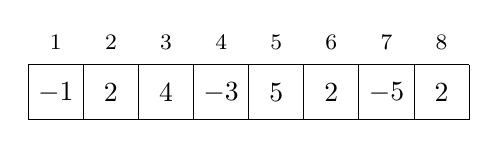
\begin{tikzpicture}[scale=0.7]
\draw (0,0) grid (8,1);

\node at (0.5,0.5) {$-1$};
\node at (1.5,0.5) {$2$};
\node at (2.5,0.5) {$4$};
\node at (3.5,0.5) {$-3$};
\node at (4.5,0.5) {$5$};
\node at (5.5,0.5) {$2$};
\node at (6.5,0.5) {$-5$};
\node at (7.5,0.5) {$2$};

\footnotesize
\node at (0.5,1.4) {$1$};
\node at (1.5,1.4) {$2$};
\node at (2.5,1.4) {$3$};
\node at (3.5,1.4) {$4$};
\node at (4.5,1.4) {$5$};
\node at (5.5,1.4) {$6$};
\node at (6.5,1.4) {$7$};
\node at (7.5,1.4) {$8$};
\end{tikzpicture}
\end{center}
\begin{samepage}
the following subarray produces the maximum sum $10$:
\begin{center}
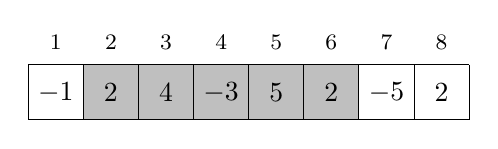
\begin{tikzpicture}[scale=0.7]
\fill[color=lightgray] (1,0) rectangle (6,1);
\draw (0,0) grid (8,1);

\node at (0.5,0.5) {$-1$};
\node at (1.5,0.5) {$2$};
\node at (2.5,0.5) {$4$};
\node at (3.5,0.5) {$-3$};
\node at (4.5,0.5) {$5$};
\node at (5.5,0.5) {$2$};
\node at (6.5,0.5) {$-5$};
\node at (7.5,0.5) {$2$};

\footnotesize
\node at (0.5,1.4) {$1$};
\node at (1.5,1.4) {$2$};
\node at (2.5,1.4) {$3$};
\node at (3.5,1.4) {$4$};
\node at (4.5,1.4) {$5$};
\node at (5.5,1.4) {$6$};
\node at (6.5,1.4) {$7$};
\node at (7.5,1.4) {$8$};
\end{tikzpicture}
\end{center}
\end{samepage}

\subsubsection{Algorithm 1}

A straightforward algorithm to the problem
is to go through all possible ways to
select a subarray, calculate the sum of
numbers in each subarray and maintain
the maximum sum.
The following code implements this algorithm:

\begin{lstlisting}
int p = 0;
for (int a = 1; a <= n; a++) {
    for (int b = a; b <= n; b++) {
        int s = 0;
        for (int c = a; c <= b; c++) {
            s += x[c];
        }
        p = max(p,s);
    }
}
cout << p << "\n";
\end{lstlisting}

The code assumes that the numbers are stored in an array \texttt{x}
with indices $1 \ldots n$.
The variables $a$ and $b$ determine the first and last
number in the subarray,
and the sum of the numbers is calculated to the variable $s$.
The variable $p$ contains the maximum sum found during the search.

The time complexity of the algorithm is $O(n^3)$,
because it consists of three nested loops and
each loop contains $O(n)$ steps.

\subsubsection{Algorithm 2}

It is easy to make the first algorithm more efficient
by removing one loop from it.
This is possible by calculating the sum at the same
time when the right end of the subarray moves.
The result is the following code:

\begin{lstlisting}
int p = 0;
for (int a = 1; a <= n; a++) {
    int s = 0;
    for (int b = a; b <= n; b++) {
        s += x[b];
        p = max(p,s);
    }
}
cout << p << "\n";
\end{lstlisting}
After this change, the time complexity is $O(n^2)$.

\subsubsection{Algorithm 3}

Surprisingly, it is possible to solve the problem
in $O(n)$ time, which means that we can remove
one more loop.
The idea is to calculate for each array position
the maximum sum of a subarray that ends at that position.
After this, the answer for the problem is the
maximum of those sums.

Consider the subproblem of finding the maximum-sum subarray
that ends at position $k$.
There are two possibilities:
\begin{enumerate}
\item The subarray only contains the element at position $k$.
\item The subarray consists of a subarray that ends
at position $k-1$, followed by the element at position $k$.
\end{enumerate}

Our goal is to find a subarray with maximum sum,
so in case 2 the subarray that ends at position $k-1$
should also have the maximum sum.
Thus, we can solve the problem efficiently
when we calculate the maximum subarray sum
for each ending position from left to right.

The following code implements the algorithm:
\begin{lstlisting}
int p = 0, s = 0;
for (int k = 1; k <= n; k++) {
    s = max(x[k],s+x[k]);
    p = max(p,s);
}
cout << p << "\n";
\end{lstlisting}

The algorithm only contains one loop
that goes through the input,
so the time complexity is $O(n)$.
This is also the best possible time complexity,
because any algorithm for the problem
has to examine all array elements at least once.

\subsubsection{Efficiency comparison}

It is interesting to study how efficient 
algorithms are in practice.
The following table shows the running times
of the above algorithms for different
values of $n$ in a modern computer.

In each test, the input was generated randomly.
The time needed for reading the input was not
measured.

\begin{center}
\begin{tabular}{rrrr}
array size $n$ & algorithm 1 & algorithm 2 & algorithm 3 \\
\hline
$10^2$ & $0{,}0$ s & $0{,}0$ s & $0{,}0$ s \\
$10^3$ & $0{,}1$ s & $0{,}0$ s & $0{,}0$ s \\
$10^4$ & > $10,0$ s & $0{,}1$ s & $0{,}0$ s \\
$10^5$ & > $10,0$ s & $5{,}3$ s & $0{,}0$ s \\
$10^6$ & > $10,0$ s & > $10,0$ s & $0{,}0$ s \\
$10^7$ & > $10,0$ s & > $10,0$ s & $0{,}0$ s \\
\end{tabular}
\end{center}

The comparison shows that all algorithms
are efficient when the input size is small,
but larger inputs bring out remarkable
differences in running times of the algorithms.
The $O(n^3)$ time algorithm 1 becomes slow
when $n=10^4$, and the $O(n^2)$ time algorithm 2
becomes slow when $n=10^5$.
Only the $O(n)$ time algorithm 3 processes
even the largest inputs instantly.
